\begin{pro}
  Modify the code \verb|demo_elliptic_fem_p1.m| to solve the following
  diffusion equation
  \begin{displaymath}
    \nabla\cdot(\kappa(x,y)\nabla u) = f(x, y) \text{ in } \Omega,
  \end{displaymath}
  with
  \begin{itemize}
  \item
    nonconstant coefficient $\kappa(x, y) = 1+xy^2$;
  \item
    analytic solution $u(x, y) = xy(1-x)(1-y), u=0$ on the boundary;
  \item
    right hand side
    \begin{displaymath}
      f(x, y) = -y^3+y^4+4y^3x-4y^4x+2y-2y^2-2x^2y+6x^2y^2+2x^3y
      - 6x^3y^2 + 2x - 2x^2.
    \end{displaymath}
  \end{itemize}
\end{pro}
\begin{sol}
  The following shows a modification of \verb|demo_elliptic_fem_p1.m|.
\begin{verbatim}
fun_D = @(x,y) 1+x.*y.^2;
fun_r = @(x,y) zeros(size(x));                       % reaction term
fun_f = @(x,y) -y.^3+y.^4+4*y.*y.*y.*x-4*y.*y.*y.*y.*x+2*y ...
    - 2*y.^2-2*x.*x.*y+6*x.*x.*y.*y+2*x.*x.*x.*y ...
    - 6*x.*x.*x.*y.*y+2*x-2*x.^2;
fun_u = @(x,y) x.*y.*(1-x).*(1-y);        %  Analyt
fun_g = @(x,y) x.*y.*(1-x).*(1-y);        %  Dirichlet boundary
\end{verbatim}
  Run the code and we obtain the following result:
    \begin{figure}[H]
    \centering
    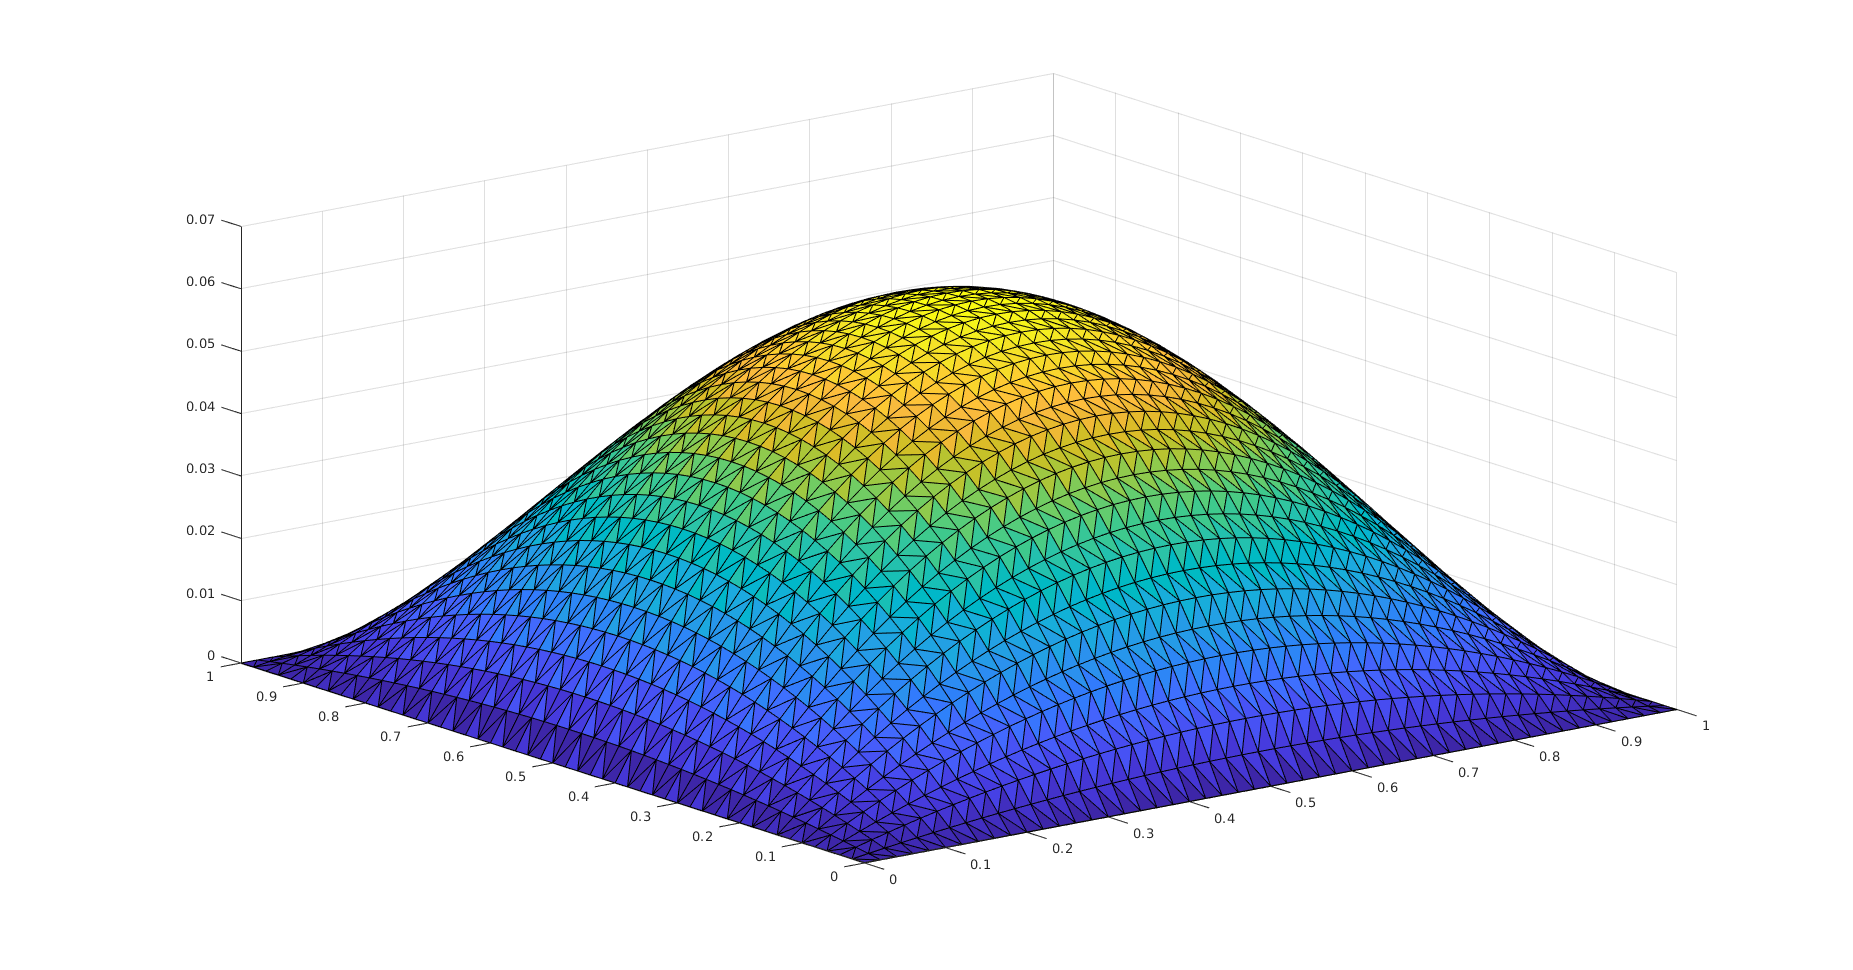
\includegraphics[scale=0.32]{png/fem.png}
  \end{figure}
\end{sol}
%%% Local Variables:
%%% mode: latex
%%% TeX-master: "../hw5"
%%% End:
